
\documentclass[11pt,a4paper]{article}
\usepackage[hyperref]{naaclhlt2019}
\usepackage{times}
\usepackage{latexsym}
\usepackage{graphicx}
\usepackage[normalem]{ulem}
\usepackage{float}
\usepackage{url}
\hbadness=99999
\aclfinalcopy 


\title{Few-shot Learning for Disease Identification from Descriptions}

\author{Jingxian Chen \\
  {\tt jic097@ucsd.edu} \\\And
  Xinyuan Wang \\
  {\tt xiw136@ucsd.edu} \\\And
  Hong Xu \\
  {\tt hox007@ucsd.edu} \\\And
  Xiaowei Zuo \\
  {\tt x1zuo@ucsd.edu} \\}
  
% \setlength\textwidth{16.0cm}
\date{}

\begin{document}
\maketitle

\begin{abstract}
Disease Identification based on patients' descriptions of their symptoms is of great importance, because there is still a severe shortage of doctors in less developed areas. Automatic disease identification system could significantly improve the medical efficiency. However, due to the rareness of some diseases and privacy issues, symptom description data is often insufficient for machine learning system. Therefore, this project performs few-shot learning on few-shot disease identification task using different methods including traditional models and large language models. After that, zero-shot medical text classification is also implemented to explore the representative ability of large language models. Finally, a comprehensive analysis is conducted to compare and analyse the performance of different methods and the reasons behind them.
\end{abstract}

\section{Introduction}

Disease identification based on text information, utilizing natural language processing (NLP) techniques, has gained prominence in healthcare and medical research. It shows, combined with textual data and other reports' complex analyses, a promising method to improve the result of the diagnosis. This study aims to compare and analyze the performance of various machine learning and deep learning models in medical text classification. By leveraging a labeled medical abstracts dataset, we evaluate the effectiveness of models in accuracy and running time. The textual data underwent preprocessing steps, including noise removal, tokenization, and feature extraction using techniques such as bag-of-words, and TF-IDF. We selected and trained multiple models, including Naive Bayes and Support Vector Machines as the baselines, BERT text classification, and Zero-shot method. The models were evaluated using standard performance metrics, including accuracy and running time. Experimental results show that the Zero-shot method can be effectively used to perform medical text classification tasks demonstrating higher accuracy and overall performance compared to others. Statistical analysis was conducted to illustrate in performance of the models.


\section{What you proposed vs. what you accomplished}

\begin{itemize}
\item \sout{Find and prepare feasible disease classification dataset}: DONE.
\item \sout{Build Naive Bayes model (Baseline 1) and evaluate}: DONE.

\item \sout{Build SVM model (Baseline 2) and evaluate}: DONE.

\item \sout{Fine-tune BERT model and evaluate}: DONE.

\item \sout{Design new classification model based on MedCLIP encoder}: DONE.

\item \sout{Design zero-shot classification method using MedCLIP encoder}: DONE.

\item \sout{Design zero-shot classification method using ChatGPT}:  Not Done: We failed to do this because of funding limitation

%\item \sout{Build and train (specific baseline model) on collected dataset and examine its performance}: DONE
%\item \sout{Make fancy model perform better than baseline model}: NOT DONE:  We failed to do this because we only started working on our project on June 13.
\end{itemize}

% \begin{itemize}
% \item \sout{Collect and preprocess dataset}: not completed
% \item \sout{Build and train (specific baseline model) on collected dataset and examine its performance}
% \item \sout{Build and train fancy model and examine its performance}
% \item \emph{Make fancy model perform better than baseline model}: We failed to do this because we only started working on our project on May 11
% \item \sout{Perform in-depth error analysis to figure out what kinds of examples our approach struggles with}
% \end{itemize}


\section{Related work}

Disease identification from text descriptions is a typical text classification task, which aims to classify given texts into different categories. It is a fundamental tasks in Natural Language Processing (NLP) area, which has been widely studied \cite{li2021survey}. In Journal of the American Medical Informatics Association, it is shown that NLP has the potential as a clinical tool for accurate and efficient prediction and classification of disease statuses from clinical summaries applied in Clinical Data—the i2b2 obesity challenge \cite{10.1197/jamia.M3096}.\\




\noindent In the late 19th century, traditional methods based on statistics dominant this area, such as Naive Bayes \cite{AutoIndex} and Supported Vector Machine (SVM) \cite{TextSVM}. Specifically, Naive Bayes calculates conditional probabilities of words given class labels assuming each word is independent of others. The naive Bayes algorithm is simple for implementation and computationally efficient, but it suffers from lacking context. On the other hand, a more computationally expensive method, SVM is efficient to handle high-dimensional features by looking for supported vectors to split the hyperspace of the given data and thus achieve great performance in classification tasks. \\

\noindent However, in 2003, Yoshua Bengio and his colleagues proposed the first deep learning model in NLP \cite{Bengio}, and then deep learning methods gradually stepped onto the stage of NLP. In 2006, Convolutional Neural Network (CNN), which is good at learning from sequential data, was introduced into text classification \cite{multitask}. Then recursive structure based model like Recursive neural networks (RNN) \cite{socher-etal-2013-recursive} and Long-short term memory networks (LSTM) were introduced to text classification because of their ability of extracting and preserving information in long sequential data. \\

\noindent Later, attention mechanism came out and soon became the most dominant backbone model structure  in NLP because of its great feature extraction power by assigning attention weight to the sequential data \cite{vaswani2017attention}. Then large language models, such as BERT \cite{devlin2019bert} and GPT \cite{Radford2018ImprovingLU} came out and showed great performance on multiple tasks including text classification. Fine-tuning the pre-trained large language model on the downstream tasks became a popular pipeline. Recently, foundation models, such as GPT3.5 \cite{brown2020language} and GPT4 \cite{openai2023gpt4}, came out by training on billions of data and adapted instruction fine-tuning, even with human-based Reinforcement Learning. These models show great representative power on plenty of tasks and inspired a brand new pipeline called prompt learning. With the help of these large models, zero-shot classification based on prompt without any need of training became possible \cite{gao2021making}.\\

\noindent The method of disease identification also followed the trend of development. The process of identifying diseases has evolved along with advancements in technology. ICU procedures and diagnosis, and medical text related documents have been addressed using Naive Bayes classification, maximum entropy classification \cite{tripathy2017document} and SVM \cite{marafino2014n}, yielding satisfactory outcomes. As deep learning techniques have progressed, several neural network models have been applied in medical text classification tasks. Convolutional Neural Networks \cite{hughes2017medical}, which has an ability to learn high-level features, shows competitive outcomes in the field of online medical guidance. On the other hand, Recurrent Neural Networks (LSTM recurrent neural networks \cite{lipton2015learning}, Bidirectional RNN \cite{jagannatha2016bidirectional}) have achieved state-of-the-art performances in clinical tasks.\\

\noindent NLP application in the medical field has shown its potential as Clinical Decision Support (CDS) which helps health professionals make clinical decisions, deal with medical data about patients or with the knowledge of drugs needed to interpret the data \cite{DBLP:journals/corr/abs-1802-05365}. Weissler et al. utilized clinical notes for identification of peripheral artery disease using a machine learning based method. The authors hypothesized that the unstructured narrative would add richer and more varied context than administrative data alone, leading to improved performance of NLP over a structured data-based approach to patient identification \cite{wei1}. In other studies, NLP application to electronic health records has been shown to add value to clinical research in multiple ways, including defining new disease phenotypes \cite{doi:10.1126/scitranslmed.aaa9364}, identifying patients for inclusion \cite{HASSANZADEH2020103406}, and extracting real-world data for analysis \cite{Fonferko-Shadrache023232}.\\

\noindent Given the previous studies on the medical data combined with the prospects of few-shot learning, we propose to evaluate various NLP models on a small scale medical dataset to test their performance on the medical domain.



\section{Your dataset}
The dataset is a medical abstracts dataset, which
describe 5 different classes of patinet conditions.
It’s created by Schopf, Tim and Braun, Daniel
and Matthes, Florian, and using it in Evaluating
Unsupervised Text Classification: Zero-shot and
Similarity-based Approaches (Zhang et al., 2022).\\

\noindent The number of data in the training set is 11550
rows and 2888 rows in the testing set. Each rows
contains 2 information: medical abstract and label.
It’s an open source dataset and easily approachable. The dataset is sufficient large ,and
notrivial. Therefore, It used as a resource to analyze the performance of models. The numerical information is shown in the table below.\\
\begin{table}[ht]
\resizebox{0.7\textwidth}{!}{\begin{minipage}{\textwidth}
\begin{tabular}{|l|l|l|l|}
\hline
                          & Mean Length & Min Length & Max Length \\ \hline
Training Set               & 1229.104                             & 170 &3999      \\ \hline
Testing Set                        & 1236.908                                & 186  &3542    \\ \hline

\end{tabular}
\end{minipage}}
\end{table}


\begin{figure}[h]
    \centering
    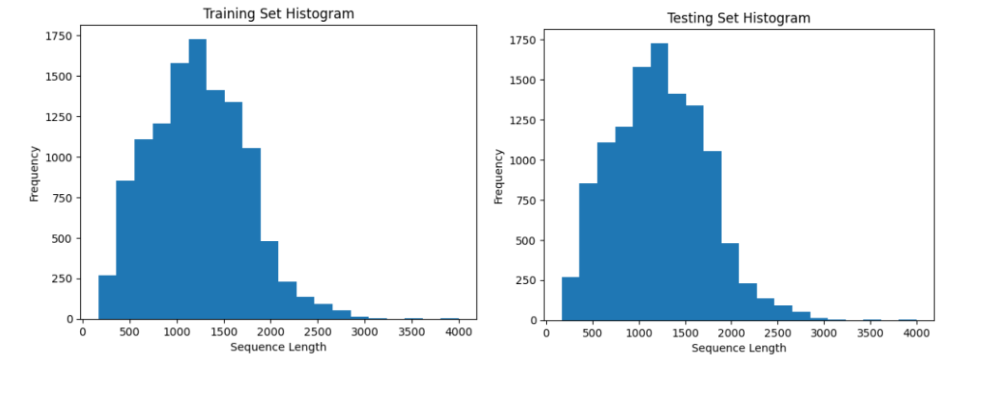
\includegraphics[width=0.5\textwidth]{Data_set_an.png}
    \caption{Visualization of Medical Abstracts Dataset}
    \label{fig:example}
\end{figure}



\subsection{Data preprocessing}
We eliminated stopwords from the corpus, stopwords in English are words that do not significantly contribute to the understanding of a sentence, their removal doesn't compromise the overall interpretation of the sentence. Also, we removed special characters like square brackets and other noisy text like URLs. Additionally, we remove the examples without labels.


% \subsection{Data annotation}
% If your project involves annotation, you may have started a pilot annotation experiment, annotating a few dozen or few hundred examples. What major issues have come up? Do you and your project partners agree or disagree on examples? Report interannotator agreement if applicable.

\section{Baselines}
What are your baselines,
Additionally, explain how each one works, and list the hyperparameters you used and how you tuned them. Describe your train/validation/test split. If you have tuned any hyperparameters on your test set, expect a major point deduction. 

\section{Your approach}
Here is a  list of things to include under this section.
\begin{itemize}
    \item  (CONCEPTUAL APPROACH) What is your approach and how does it work? 
    \item  (WORKING IMPLEMENTATION) Did you manage to complete a working implementation?
   \item (OTHER PEOPLE'S CODE)  Did you rely on help from any existing implementations? If so, please link to them here. 
   \item  (IMPLEMENTATION) \textbf{What models did you implement yourself, and what files in your submitted code are associated with these models?} ( there will be a code submission link)
   \item (COMPUTE) What kind of computers are you running your experiments on? Are there any issues that you could not solve? If you used Colab, were there any Colab-specific hacks you needed to make to train your model? 

   \item (RUNTIME) How long did it take to train your model?

   \item  (RESULTS) What results did your model achieve, and how do these results compare to your baselines? 

   \item (OTHER): There could be many other important details specific to your approach that you should include here if appropriate. 
\end{itemize}
% Do you expect it to fail in similar ways to your baselines? What libraries did you use to accomplish this? \textbf{What models did you implement yourself, and what files in your uploaded code are associated with these models?} What kind of computers are you running your experiments on? Are there any issues that you could not solve? If you used Colab, were there any Colab-specific hacks you needed to make to train your model? What results did your model achieve, and how do these results compare to your baselines? Be specific!!! Note that there could be many other important details specific to your approach that you should include here if appropriate.

\section{Error analysis}
What kinds of inputs do your baselines fail at? What about your approach? Are there any semantic or syntactic commonalities between these difficult examples? \textbf{We would like to see a manual error analysis (e.g., annotate about some failed examples for various properties, and then discuss the results and hypothesize about why the ).} 

\section{Contributions of group members}
List what each member of the group contributed to this project here. For example: 
\begin{itemize}
    \item member 1: did data collection / processing and lots of writing
    \item member 2: built and trained models
    \item member 3: error analysis and annotations
\end{itemize}

\textit{ \color{blue} If you would like to privately share more information about the workload division that may have caused extenuating circumstances (e.g., a member of the group was unreachable and did no work), please send a detailed note to the instructor. We will take these notes into account when assigning individual grades.}


\begin{table*}
\begin{center}
\begin{tabular}{|l|l|l|l|}
\hline
                          & Traning Time Per Epoch (Minutes) & Evaluation Time (Minutes) & Test Accuracy \\ \hline
Naive Bayes               & 0.029                            & 0.001                     & 0.579986      \\ \hline
SVM                       & 2                                & 0.5                       & 0.557479      \\ \hline
BERT                      & 10                               & 1                         & 0.636773      \\ \hline
MedCLIP (Fine-tune based) & 0.45                             & 0.05                      & 0.593333      \\ \hline
MedCLIP (Zero-shot based) & N/A                              & 1                         & 0.972401      \\ \hline
\end{tabular}
\end{center}
\end{table*}


\section{Conclusion}
You've now gotten your hands dirty with NLP tools and techniques! What takeaways do you have about your project? What proved surprisingly difficult to accomplish? Were your surprised by your results? If you could continue working on your project in the future, what directions would you pursue?


\bibliographystyle{apalike}
\footnotesize
\bibliography{yourbib}



\end{document}
